\documentclass[11pt]{article}
\usepackage[review]{acl}
\usepackage{times}
\usepackage{latexsym}
\usepackage[T1]{fontenc}
\usepackage[utf8]{inputenc}
\usepackage{microtype}
\usepackage{inconsolata}
\usepackage{booktabs}
\usepackage{amsmath}
\usepackage{array}
\usepackage{tabularx}
\usepackage{graphicx}
\usepackage{float}
\usepackage[section]{placeins}

\newcolumntype{Y}{>{\raggedright\arraybackslash}X}

\title{A Reproducibility-Oriented Critique of BLIP-2, LLaVA, and VisionLLM v2\\
with a Local-Scale BLIP-2 Reproduction}
\author{Anonymous}

\begin{document}
\maketitle

\begin{abstract}
Multimodal large language models combine pretrained visual encoders, language models,
and cross-modal alignment modules, but faithful reproduction of published systems
remains difficult outside large compute environments. This paper studies three
representative systems---BLIP-2, LLaVA, and VisionLLM v2---to identify where the
main technical gains come from and where the principal reproducibility barriers
remain. The comparative questions are threefold: which of the three systems is the
most suitable target for local implementation, which design choices remain
meaningful after aggressive downscaling, and how much of the observed performance
gap is attributable to scale rather than to pipeline failure. To answer these
questions, the study combines a structured critique of the three papers with a local
reproduction of BLIP-2 using the official LAVIS codebase, reduced COCO Karpathy
subsets, CLIP ViT-L, and OPT-350M on a single RTX 3070 8GB GPU. The reproduction
completes stage-1 representation learning, stage-2 generative alignment, and caption
fine-tuning. The best local result is obtained on a 50k/1k/1k split, reaching
BLEU-4 11.13 and CIDEr 37.57, while a larger 100k run peaks early at epoch 2 and
does not surpass the 50k best. The main finding is that BLIP-2 is the most
defensible local reproduction target among the three papers and is reproducible at the
pipeline level, but its captioning quality remains strongly constrained by backbone
scale, optimization budget, and evaluation setting.
\end{abstract}

\section{Introduction}
Recent multimodal large language models (MLLMs) have expanded the scope of
vision-language research from captioning and visual question answering to
instruction-following assistants, grounding, segmentation, generation, and editing.
This progress has been driven by the combination of large pretrained vision
encoders, large language models, and increasingly sophisticated alignment modules.
At the same time, the field has become substantially harder to reproduce. Strong
reported results are now often inseparable from large-scale pretraining corpora,
multi-stage optimization, and extensive compute budgets, which makes it difficult to
separate architectural contribution from scale advantage.

This tension is especially visible across three influential papers that occupy
different points in the current design space. BLIP-2 introduces a modular
Querying Transformer (Q-Former) that connects a frozen image encoder to a frozen
language model through a compact trainable bridge \citep{li2023blip2}. LLaVA shifts
the emphasis toward assistant behavior by aligning a vision encoder and a Vicuna-like
language model through multimodal instruction tuning \citep{liu2023visual}. VisionLLM
v2 pushes further toward a generalist system that routes a central multimodal model
into multiple task-specific decoders for perception and generation
\citep{wu2024visionllmv2}. In parallel, adjacent bridge-based work such as Flamingo
and the original BLIP highlights a broader research trend: increasingly capable
multimodal systems are being built by reusing strong unimodal backbones rather than
training every component from scratch \citep{alayrac2022flamingo,li2022blip}.

The research gap addressed here is not simply whether these systems are strong, since
their benchmark performance is already well established, but which aspects of their
design remain reproducible and interpretable under local constraints. Existing
papers report impressive empirical results, yet they do not directly answer the
practical question that matters for a constrained implementation study: which model
offers the best balance of novelty, openness, compute realism, and scientific
interpretability when scaled down to commodity hardware? A second gap concerns
pipeline fidelity. Even when official code is available, it is often unclear whether
the full training path can be executed end-to-end on a local system without changing
the method itself.

This paper addresses three questions. First, which of BLIP-2, LLaVA, and VisionLLM
v2 offers the strongest local reproducibility profile? Second, once BLIP-2 is
selected, can its official staged training pipeline be executed end-to-end on a
single consumer GPU using principled downscaling rather than ad hoc simplification?
Third, under a fixed local architecture, how does caption quality evolve as the data
scale increases from 10k to 50k to 100k COCO training examples?

The paper answers these questions through a two-part methodology. The first part is a
structured critique of the three papers, organized around problem formulation, core
technical idea, methodology, experimental setup, results, and reproducibility
implications. The second part is a local BLIP-2 reproduction based on the
official LAVIS implementation, reduced COCO Karpathy subsets, CLIP ViT-L,
\texttt{facebook/opt-350m}, and a single NVIDIA RTX 3070 8GB GPU. The implementation
uses the same three-stage training logic as the original method, with targeted
engineering adaptations for a local Windows environment and a subset-matched offline
evaluation path for BLEU and CIDEr.

The main contributions are fourfold. First, the paper provides a
reproducibility-aware critique of three representative MLLM papers rather than
treating paper selection as a brief preface to implementation. Second, it documents a
complete local BLIP-2 reproduction that preserves the official staged training
structure. Third, it presents a controlled scaling analysis across 10k, 50k, and 100k
training examples under a fixed architecture. Fourth, it shows that BLIP-2 is
reproducible at the pipeline level on local hardware, but that its captioning
performance remains strongly constrained by scale.

\section{Comparative Critique of the Three Papers}

\subsection{BLIP-2}
\paragraph{Problem and motivation.}
BLIP-2 addresses a central problem in multimodal learning: large language models and
large vision encoders are already strong individually, but jointly training a
multimodal system around them is computationally expensive and often redundant.
The paper is motivated by the question of whether a lightweight trainable interface can
reuse frozen unimodal backbones while retaining strong downstream performance
\citep{li2023blip2}.

\paragraph{Key idea and approach.}
The core idea is the Q-Former, a compact transformer that mediates between a frozen
image encoder and a frozen language model. Rather than finetuning the full
multimodal stack, the method learns a small set of query-conditioned visual features
that are projected into the language-model input space. This bottleneck is the paper's
main conceptual strength because it yields a precise architectural hypothesis: a
carefully trained bridge may be sufficient to connect strong frozen backbones.

\paragraph{Methodology.}
The method uses two major training stages. Stage 1 trains the Q-Former against the
frozen image encoder using image-text contrastive learning, image-text matching, and
language modeling. Stage 2 aligns the Q-Former outputs to a frozen language model for
generation. The architecture is modular, the gradient flow is interpretable, and the
training objectives are clearly separated by function.

\paragraph{Dataset and experimental setup.}
The full paper uses a 129M image-text pretraining mixture assembled from COCO,
Visual Genome, CC3M, CC12M, SBU, and LAION subsets, followed by downstream evaluation
and finetuning on established benchmarks \citep{li2023blip2}. The strongest reported
configurations use large frozen backbones such as ViT-g and OPT-2.7B, with training
performed on a 16-A100(40GB) machine for multiple days.

\paragraph{Results.}
BLIP-2 reports strong zero-shot and finetuned results across VQA, captioning, and
retrieval. A particularly striking result is that it surpasses Flamingo-80B on
zero-shot VQAv2 by 8.7 absolute points while using 54$\times$ fewer trainable
parameters \citep{li2023blip2}. On COCO captioning, the reported ViT-g OPT-2.7B
configuration reaches BLEU-4 43.7 and CIDEr 145.8.

\paragraph{Main takeaways.}
BLIP-2 is the strongest local reproduction target among the three papers because its method
remains scientifically coherent after downscaling. However, the paper's
``compute-efficient'' framing is relative to prior frontier systems, not to commodity
hardware. The method is modular and reproducible in principle, but paper-level
performance remains tightly coupled to large data and backbone scale.

\subsection{LLaVA}
\paragraph{Problem and motivation.}
LLaVA addresses a different problem: multimodal systems may recognize images, yet still
behave poorly as assistants because they are not trained on conversational and
instruction-following supervision. The paper is motivated by the need for a practical,
open visual assistant rather than by a new bridge architecture alone
\citep{liu2023visual}.

\paragraph{Key idea and approach.}
The central idea is simple and influential: a frozen CLIP image encoder can be linked
to a Vicuna-style language model through a lightweight projection layer, after which
the combined model can be trained on multimodal instruction-following data. The paper's
main contribution is therefore data-centric rather than deeply architectural.

\paragraph{Methodology.}
LLaVA uses a two-step procedure: feature alignment between the vision encoder and the
language model, followed by visual instruction tuning. The instruction data are
generated by GPT-4 from symbolic image descriptions, and the training set contains
158K multimodal instruction-response pairs \citep{liu2023visual}. The design is
methodologically appealing because it demonstrates how much assistant-like behavior can
be induced by supervision format.

\paragraph{Dataset and experimental setup.}
The paper uses CLIP ViT-L as the visual backbone and Vicuna as the language model, with
training conducted on 8 A100 GPUs. The reported instruction-tuning phase completes in
roughly 10 hours \citep{liu2023visual}, which is considerably more accessible than the
largest BLIP-2 pretraining setup, although still well beyond a single 8GB consumer GPU.

\paragraph{Results.}
LLaVA demonstrates strong open-ended conversational behavior and reports state-of-the-art
performance on ScienceQA when combined with GPT-4 as a judge, reaching 92.53\%
\citep{liu2023visual}. The paper's impact is also visible historically: it established
visual instruction tuning as a dominant pattern in open-source multimodal assistant
research.

\paragraph{Main takeaways.}
LLaVA is compelling because it reorients the problem from representation learning to
alignment and supervision. Its main limitation, from a reproduction perspective, is
that a large part of its success is entangled with the GPT-generated instruction
pipeline. The architecture is comparatively simple, but faithful reproduction depends on
recreating the data-generation strategy.

\subsection{VisionLLM v2}
\paragraph{Problem and motivation.}
VisionLLM v2 targets the broadest problem of the three papers: most multimodal systems
remain narrow, producing primarily text outputs while relying on separate specialist
models for detection, segmentation, pose estimation, and generation. The paper is
motivated by the goal of a single end-to-end generalist system for many vision and
vision-language tasks \citep{wu2024visionllmv2}.

\paragraph{Key idea and approach.}
Its central mechanism is the ``super link,'' which combines routing tokens and
task-specific learnable queries to connect a core multimodal language model to multiple
external decoders. This design enables end-to-end gradient flow from task-specific
objectives back into the shared model, which is more ambitious than a tool-use style
interface.

\paragraph{Methodology.}
The methodology is multi-stage and multi-decoder. The system integrates decoders such
as Grounding DINO, UniPose, Stable Diffusion v1.5, and InstructPix2Pix, and trains the
overall model across a very broad task set \citep{wu2024visionllmv2}. The resulting
system is impressive, but methodologically harder to isolate because gains may derive
from routing, decoder reuse, data scale, or task breadth.

\paragraph{Dataset and experimental setup.}
The experimental setup is the most demanding of the three papers. The appendix reports
64 A100(80GB) GPUs for stage 1 and 128 A100 GPUs for later stages, with total training
time on the order of 18 days \citep{wu2024visionllmv2}. The system also depends on
multiple pretrained decoders and a large collection of datasets and task templates.

\paragraph{Results.}
VisionLLM v2 reports broad generalist capability and competitive specialist performance.
For example, it reports 56.7 AP$_b$ on COCO object detection with a Swin-T backbone,
competitive with Grounding-DINO-T, along with strong results in pose and segmentation
settings \citep{wu2024visionllmv2}. Its contribution is therefore breadth more than a
single benchmark win.

\paragraph{Main takeaways.}
VisionLLM v2 is an important systems contribution, but it is not a viable local
reproduction target for this study. Its engineering complexity and compute requirements
are too high for local implementation, and its scientific contribution is more
difficult to disentangle cleanly under heavy downscaling.

\begin{table}[t]
\centering
\scriptsize
\setlength{\tabcolsep}{3pt}
\begin{tabularx}{\linewidth}{p{1.5cm} Y Y Y Y}
\toprule
Paper & Problem focus & Central idea & Experimental scale & Local reproduction verdict \\
\midrule
BLIP-2 & Connect frozen vision and language backbones efficiently for multimodal generation and understanding & Two-stage Q-Former bridge between a frozen image encoder and a frozen LLM & 129M image-text pairs; multi-day training on 16 A100 GPUs for large variants & Best target: modular, open, and interpretable after downscaling \\
LLaVA & Build a practical multimodal assistant rather than only a captioning or representation model & Lightweight vision-language projection plus multimodal instruction tuning & 8 A100 GPUs; GPT-generated instruction data; moderate but still non-local compute & Viable only with stronger hardware and the instruction-data pipeline \\
VisionLLM v2 & Unify many vision and vision-language tasks inside one end-to-end system & Super-link routing between a central MLLM and multiple specialist decoders & 64--128 A100 GPUs; multi-stage training across many tasks and decoders & Not viable for a local reproduction study \\
\bottomrule
\end{tabularx}
\caption{Comparative summary of the three papers from a reproducibility-oriented perspective.}
\label{tab:critique-summary}
\end{table}

\section{Local BLIP-2 Reproduction}
The reproduction focuses on technical execution rather than on reiterating the model
selection argument. The objective is to preserve the official staged BLIP-2 training
logic while aggressively reducing scale so that the full pipeline can run on a single
RTX 3070 8GB GPU. Success is therefore defined at the pipeline level: valid completion
of stage 1, stage 2, and caption finetuning, together with reproducible evaluation on a
fixed local benchmark. The completed runs should be read as successive attempts within
one local reproduction, not as separate environments: a 10k pilot attempt, a 50k main
attempt with a short 50k refinement rerun, and a 100k long-run attempt.

\subsection{Pipeline and Mathematical Formulation}
BLIP-2 consists of three components: a frozen vision encoder $E_v$, a trainable
Q-Former $Q_\theta$, and a frozen language model $E_l$ \citep{li2023blip2}. Given an
image $x$, the vision encoder produces visual features $V = E_v(x)$. A fixed set of
learned query tokens interacts with $V$ through the Q-Former to produce
query-conditioned outputs
\[
Z = Q_\theta(V).
\]
These outputs are projected into the language-model input space through a learned
projection matrix $W$, producing the soft visual prompts that condition generation.

Stage 1 trains the bridge against the frozen image encoder using the same local LAVIS
objective family as the official implementation:
\[
\mathcal{L}_{\text{stage1}} =
\mathcal{L}_{\text{itc}} +
\mathcal{L}_{\text{itm}} +
\mathcal{L}_{\text{lm}}.
\]
Here, $\mathcal{L}_{\text{itc}}$ enforces image-text contrastive alignment,
$\mathcal{L}_{\text{itm}}$ trains a matching classifier over fused representations, and
$\mathcal{L}_{\text{lm}}$ encourages the bridge to support caption-token prediction.

Stage 2 aligns the bridge to the frozen language model through an autoregressive
objective:
\[
\mathcal{L}_{\text{stage2}} =
- \sum_{t=1}^{T} \log p(y_t \mid y_{<t}, WZ),
\]
where $y$ denotes the target caption tokens. Caption finetuning uses the same
image-conditioned generative path but specializes it to COCO captioning with the prompt
\texttt{a photo of}. The local configuration keeps 32 query tokens throughout.

\subsection{Local Data, Configuration, and Evaluation Protocol}
The local benchmark is derived from deterministic subsets of the COCO Karpathy caption
splits \citep{lin2014coco}. Three training scales are used: 10k/1k/1k, 50k/1k/1k, and
100k/1k/1k for train/validation/test. Validation and test remain fixed at 1,000 images
across all runs so that internal comparisons reflect model behavior rather than split
changes.

The local model uses CLIP ViT-L as the visual backbone, OPT-350M as the language model,
image resolution 224, 32 query tokens, automatic mixed precision, and gradient
accumulation of 8. The 50k attempt family uses a 3/3/5 schedule for stages 1, 2, and
caption finetuning, while the 100k long-run attempt uses a 10/10/15 schedule.
Evaluation is performed offline because the stock Windows METEOR path was unstable in
the local environment. The checkpoint-producing caption runs therefore use
\texttt{report\_metric=false}, after which BLEU and CIDEr are computed from saved
\texttt{val\_epoch*.json} files against subset-matched COCO-format ground truth.

\begin{table}[H]
\centering
\scriptsize
\setlength{\tabcolsep}{4pt}
\begin{tabularx}{\linewidth}{p{3.2cm} Y Y}
\toprule
Dimension & BLIP-2 paper configuration & Local reproduction \\
\midrule
Pretraining data & 129M image-text pairs from COCO, Visual Genome, CC3M, CC12M, SBU, and LAION subsets \citep{li2023blip2} & Reduced COCO Karpathy subsets only: 10k, 50k, and 100k training examples \\
Bridge schedule & 250k steps in stage 1 and 80k steps in stage 2 \citep{li2023blip2} & 3 epochs / 3 epochs in the 50k attempts; 10 epochs / 10 epochs in the 100k long run \\
Caption setup & 5 epochs, batch size 256, image resolution 364 \citep{li2023blip2} & 5 caption epochs in the 50k attempts or 15 in the 100k long run, batch size 1--2 with accumulation 8, image resolution 224 \\
Vision encoder & ViT-g/14 for the strongest OPT caption result \citep{li2023blip2} & CLIP ViT-L \\
Language model & OPT-2.7B \citep{li2023blip2} & OPT-350M \\
Compute & Multi-day training on 16 A100 GPUs for large variants \citep{li2023blip2} & One RTX 3070 8GB GPU; multi-hour to multi-day desktop runs \\
\bottomrule
\end{tabularx}
\caption{Original BLIP-2 scale and the local reproduction.}
\label{tab:setup-compare-v2}
\end{table}

\subsection{Implementation Adaptations}
The reproduction retains the official LAVIS code path, but several targeted engineering
adaptations are required to make it reliable in a local Windows setting. First,
non-distributed guards are added around collective operations and barriers so that the
training loop functions in single-process mode. Second, the local OPT-350M path
requires a projection fix because the Q-Former outputs must be mapped into the actual
token-embedding dimension rather than the hidden-size assumption used for larger OPT
variants. Third, local cache-path and \texttt{image\_id} fixes are required so that the
reduced COCO subsets align correctly with the evaluator. Fourth, the metric path is
reconstructed offline with subset-matched ground truth because Windows METEOR was
unstable. Fifth, per-epoch checkpoint saving and resume hooks are added so that long
runs remain recoverable and every caption epoch can be scored after training.

\subsection{Results and Comparison}
Across the completed local attempts, all three stages run successfully on the 10k
pilot, the 50k line, and the 100k long-run configuration. The 50k line includes a
main attempt and a short refinement rerun; the strongest completed local caption result
is the main attempt selected at epoch 3. This result reaches BLEU-4 11.13 and CIDEr
37.57 on the paper-style $\times 100$ scale. The 100k long-run attempt is
operationally successful and more diverse, but its best checkpoint occurs at epoch 2
and still underperforms the 50k best.

\begin{table}[H]
\centering
\small
\begin{tabular}{lrr}
\toprule
Metric & Paper & Local best \\
\midrule
BLEU-4 & 43.7 & 11.13 \\
CIDEr & 145.8 & 37.57 \\
\bottomrule
\end{tabular}
\caption{BLIP-2 paper result and the best local completed result. The values are not
directly leaderboard-equivalent because the local system uses smaller backbones, less
data, lower resolution, and a reduced validation split.}
\label{tab:paper-vs-local-v2}
\end{table}

\begin{table}[H]
\centering
\scriptsize
\setlength{\tabcolsep}{4pt}
\begin{tabular}{@{}lcrrr@{}}
\toprule
Run & Scale & BLEU-4 & CIDEr & Unique captions \\
\midrule
\texttt{10k} pilot (final e0) & \texttt{10k} & 1.45 & 3.03 & 61 \\
\texttt{50k} main (best e3) & \texttt{50k} & 11.13 & 37.57 & 563 \\
\texttt{50k} refinement (final e4) & \texttt{50k} & 10.49 & 37.14 & 607 \\
\texttt{100k} long-run (best e2) & \texttt{100k} & 8.57 & 25.34 & 677 \\
\texttt{100k} long-run (final e14) & \texttt{100k} & 6.61 & 18.36 & 734 \\
\bottomrule
\end{tabular}
\caption{Internal scaling comparison across completed local runs.}
\label{tab:internal-scaling-v2}
\end{table}

The local scaling trend is therefore clear. Increasing the training set from 10k to
50k produces a large quality gain, which indicates that the local pipeline is learning
meaningful cross-modal structure rather than emitting arbitrary captions. The transition
from 50k to 100k is different: caption diversity continues to rise, but BLEU and CIDEr
peak early and then decline.

\begin{figure}[H]
\centering
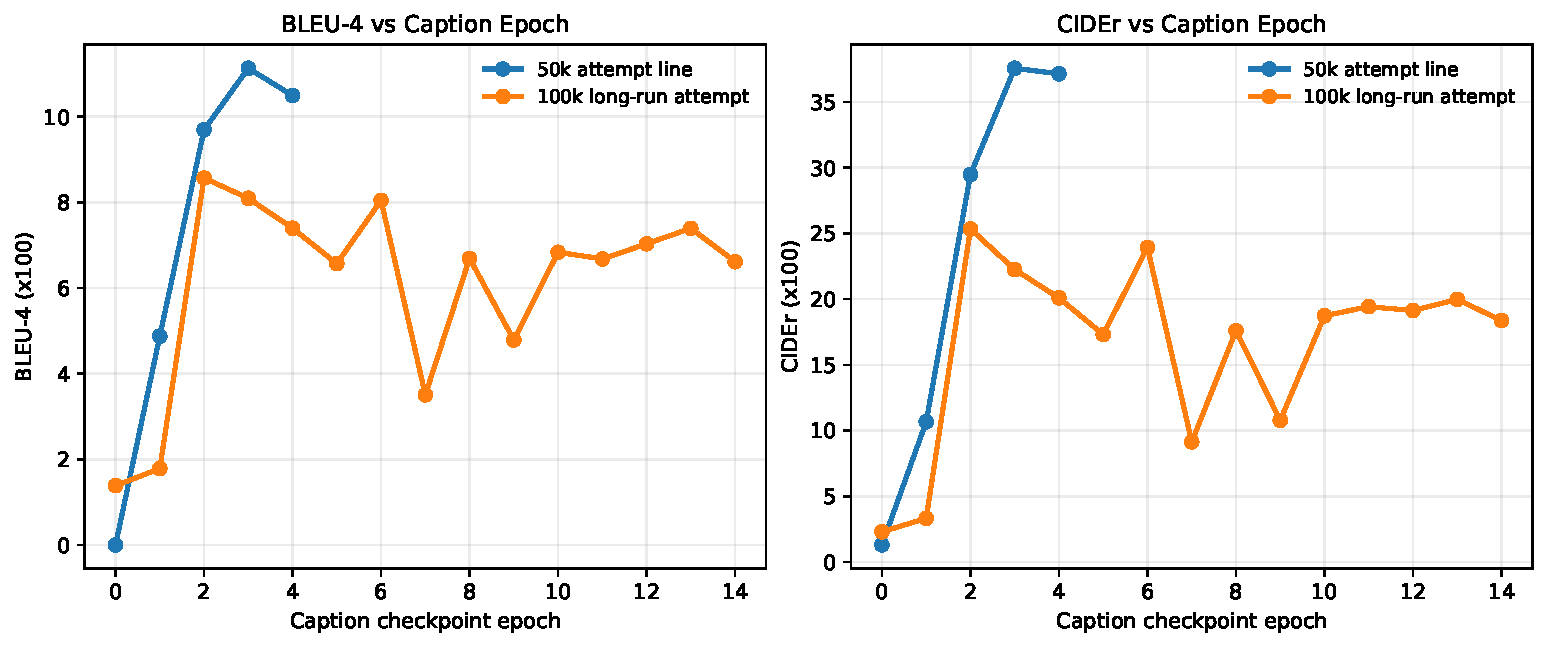
\includegraphics[width=\linewidth]{figures/caption_epoch_trajectories.pdf}
\caption{Caption metric trajectories for the completed 50k and 100k paths. The 100k
run peaks early and then degrades, so best-checkpoint selection by validation CIDEr is
empirically necessary rather than optional.}
\label{fig:caption-trajectories-v2}
\end{figure}

The training losses support the claim that the pipeline itself is functioning. The
50k main attempt ends stage 1 at loss 0.412 and stage 2 at 0.767, while the 100k
long-run attempt ends stage 1 at 0.330 and stage 2 at 0.363. Caption loss also
decreases steadily in the long run. The main failure mode therefore appears in model
selection and final caption quality rather than in the basic operability of the
training stages.

\begin{figure}[H]
\centering
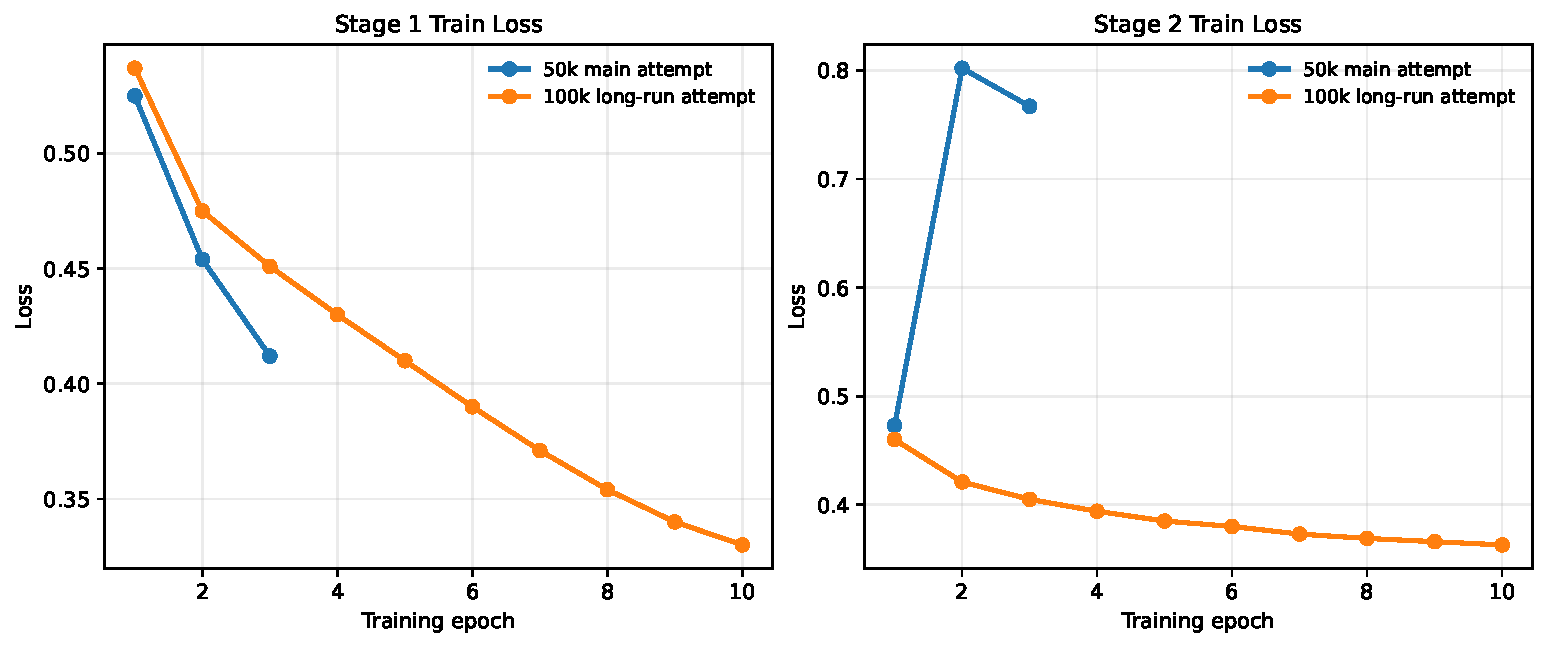
\includegraphics[width=\linewidth]{figures/training_loss_trajectories.pdf}
\caption{Stage-1 and stage-2 train-loss trajectories for the 50k and 100k runs. The
smooth loss decrease in the 100k run indicates that later caption degradation is better
interpreted as a selection or overtraining issue than as a bridge-stage instability.}
\label{fig:loss-trajectories-v2}
\end{figure}

\begin{table}[H]
\centering
\scriptsize
\begin{tabular}{lrrr}
\toprule
\texttt{100k} checkpoint & BLEU-4 & CIDEr & Unique captions \\
\midrule
Best epoch 2 & 8.57 & 25.34 & 677 \\
Final epoch 14 & 6.61 & 18.36 & 734 \\
\bottomrule
\end{tabular}
\caption{Best and final checkpoints for the 100k long run.}
\label{tab:best-final-v2}
\end{table}

Under the fixed local architecture used here, larger data and a much longer
schedule do not automatically yield better captioning quality. The evidence points to
an optimization and checkpoint-selection problem rather than a failure of the staged
BLIP-2 design itself.

\FloatBarrier

\section{Limitations and Validity}
The conclusions are informative but bounded by several limitations. The local evaluation
uses a fixed 1,000-image validation subset rather than the full Karpathy COCO test set,
so the reported numbers are directly comparable across local runs but not directly
comparable to the paper's leaderboard setting. The local architecture also differs
materially from the strongest BLIP-2 captioning configuration: CLIP ViT-L and OPT-350M
replace ViT-g and OPT-2.7B, and the image resolution is reduced from 364 to 224.

A second limitation concerns systems validity. The reproduction relies on targeted code
adaptations to make the official LAVIS path work in a single-process Windows
environment. These modifications do not change the intended training logic, but they do
mean that the study measures both model reproducibility and the portability of a
research codebase into a non-native environment. A third limitation is that all
completed runs are single-seed trajectories. The ranking between the 50k and 100k runs
is therefore empirically grounded but not variance-estimated.

\section{Discussion}
One useful distinction preserved from the larger draft is between pipeline
reproducibility and performance reproducibility. At the pipeline level, the answer is
positive: after targeted engineering fixes, the official BLIP-2 path can run end to
end on a single consumer GPU, produce recoverable checkpoints, and support stable
offline BLEU/CIDEr evaluation. At the performance level, the answer is more limited.
The local system remains far below the paper's captioning quality even after the clear
improvement from the 10k pilot to the 50k main attempt. Treating these as separate
outcomes makes the reproduction result more precise and more scientifically useful.

The project also contributes an artifact trail rather than only a final score. The
reported metrics are traceable to saved validation predictions and subset-matched
ground-truth files, and the later 50k and 100k attempts are continuations of the same
codebase rather than disconnected experiments. This matters because the 100k result
shows that schedule design and checkpoint selection matter as much as raw runtime: the
pipeline stays stable while caption quality peaks early. The work is therefore useful
not only as a numerical comparison, but also as a reusable local BLIP-2 reproduction
scaffold.

\section{Conclusion}
This paper evaluated BLIP-2, LLaVA, and VisionLLM v2 through a reproducibility-oriented
critique and then implemented a local-scale BLIP-2 reproduction on a single RTX 3070
8GB GPU. The comparative analysis shows that BLIP-2 is the most suitable target for a
local implementation study because its Q-Former architecture remains interpretable after
downscaling, whereas LLaVA depends more heavily on a synthetic instruction-data
pipeline and VisionLLM v2 depends on very large compute and decoder breadth.

The reproduction confirms that the BLIP-2 pipeline is executable end-to-end at local
scale. Stage-1 representation learning, stage-2 generative alignment, and caption
fine-tuning all complete successfully, and the local evaluation path produces stable
BLEU/CIDEr estimates from saved checkpoints. The best local result, obtained on the
50k main attempt, reaches BLEU-4 11.13 and CIDEr 37.57; the larger 100k long-run
attempt also completes successfully, but peaks early and does not surpass the 50k best.

The central conclusion is straightforward. BLIP-2 is reproducible at the pipeline
level on commodity hardware after targeted engineering work, but its published
captioning quality is not reproducible at that scale. The remaining performance gap is
best explained by backbone size, data scale, optimization budget, and evaluation
setting rather than by a failure of the staged training method itself.

\bibliography{term_paper}

\end{document}
